\documentclass[twoside,10pt]{article}
\usepackage{shlists}
\usepackage[utf8]{inputenc}
\usepackage[spanish]{babel}
\usepackage[T1]{fontenc}


\usepackage{multicol}
\usepackage{picinpar}

\usepackage{url}
\newcommand{\surl}[1]{{\small\url{#1}}}

\newcounter{vol}
\newcounter{num}
\newcounter{anyo}
\setcounter{vol}{10}
\setcounter{num}{1}
\setcounter{anyo}{2017}
\newcommand{\mes}{Enero}
\usepackage{revisionNLcol}


\title{\ \\ Docencia 2.0\\ \large Juan Julián Merelo, Fernando Tricas}
\author{\LARGE Diseñando un proyecto: {\sl design thinking} para los estudios de informática}

\date{}

\AutTit{Docencia 2.0}

\begin{document}
\addtocounter{page}{2}

\maketitle
\vspace*{-5ex}

\begin{multicols}{2}

Uno de los problemas a los que se enfrentan tanto estudiantes como el profesorado
cuando tratan de proponer nuevos proyectos para una asignatura o TFG (de los
que hablamos, por cierto, no hace tanto en la columna «En defensa de los
trabajos de fin de grado»\footnote{ReVisión, Vol 9, No 2
(2016)~\url{http://www.aenui.net/ojs/index.php?journal=revision&page=article&op=view&path[]=238&path[]=381}}), 
es encontrar un tema que sea atractivo para el estudiante, que esté dentro
de la órbita de los conocimientos de los dos y que también
lo acerque, dentro de lo posible, al mundo real, o al menos a un émulo del
mundo real suficientemente razonable. 

El cumplimiento de ese conjunto de restricciones hace que el campo
disponible se reduzca mucho: extensiones de proyectos anteriores,
proyectos en los que el estudiante esté en ese momento trabajando, si
es que está relacionado con una empresa, o pequeños proyectos
relacionados con la investigación del tutor, suelen ser las soluciones
más socorridas.  Sin embargo, no siempre se pueden cumplir todas las
restricciones y en ocasiones el requisito que se suele caer de ese
panel es el de acercarse al mundo real.  O acercarse demasiado a una
parte muy limitada de ese mundo que se reduce a los intereses de quien
realiza el proyecto o de quien lo encarga.  Lo que es una pena,
porque como ya dijimos en la columna anterior sobre TFG, proyectos
realizados, siempre que se liberen (o al menos se abran en un
repositorio), acaban formando parte de un portafolio que será la carta
de presentación del estudiante ya graduado al mundo de la empresa.  Y
el hecho de que el proyecto sea atractivo, bien pensado, con un
público objetivo definido y no solo técnicamente correcto, puede
aumentar su empleabilidad considerablemente.  Y también la diversión:
más interaccción, más variables que considerar y más oportunidades.
El problema es que un proyecto poco atractivo y sin un público
objetivo definido es difícil que sea técnicamente correcto, por lo
que una fase de elección y diseño adecuada es esencial para el éxito
del mismo.

La creación del proyecto, en sí, es una técnica y también una metodología, y
una que se puede también {\em aprobar} o {\em suspender}. Y que se
debe y hay que aprender. Un proyecto llevado a
su término pero cuyo público objetivo esté mal pensado o no exista puede dar al
traste con el esfuerzo realizado. Y para ello está la metodología denominada,
por alguna razón en inglés, {\sl design thinking}, o {\em la forma en que
  piensan los diseñadores}, una metodología que se ha impuesto
últimamente en eventos de tipo {\sl startup}, donde se trata de
diseñar una compañía alrededor de un producto diseñado de esta forma.
%Esta frase no termino de pillarla bien.
%Era una broma con el uso de términos ingleses. la quito. 
En todo caso, cuando hablamos de {\sl design thinking} estamos
pensando en resolución de tareas que requieran la aparición de un
enfoque creativo. Pero no hablamos de creatividad porque sí, sino una
creativididad dirigida a poner a las personas en el centro y sus necesidades como
objetivo. 

%--------------------------
\noindent\rule{86mm}{1pt}
\vspace{1ex} {\small{\begin{window}[0,r,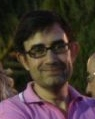
\includegraphics[width = 27mm]{JJM.jpg},] 
\noindent\emph{JJ Merelo} es catedrático de Universidad
en el área de Arquitectura y Tecnología de Computadores, y
actualmente director de la Oficina de Software Libre de la UGR.
Mantiene un blog desde el año 2002, y lo ha utilizado en clase desde
el año 2004; también wikis, agregadores y repositorios de código
como herramientas docente. Últimamente le ha dado por el \textsl{flipped
learning}, de lo que se informará debidamente en esta columna.
\end{window}}}

\medskip

{\small{\begin{window}[0,r,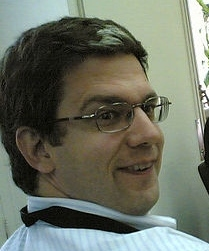
\includegraphics[width = 27 mm]{FTricas1.jpg},]
		\noindent \emph{Fernando Tricas García} es profesor
		titular de Lenguajes y Sistemas Informáticos del Departamento
		de Informática e Ingeniería de Sistemas de la Universidad de
		Zaragoza.  Empezó a estudiar la blogosfera casi cuando aún no
		existía (allá por el año 2002) y a tratar de integrarla en los
		cursos y tareas docentes un poco después.  Ha impartido
		numerosas charlas relacionadas con el tema de la Web 2.0, 
		internet y universidad,\ldots\ 
		Es actualmente Vicerrector de Tecnologías de la Información y
de la Comunicación.   
		\end{window}}}
%-------------------------------------------------

Podemos ver propuestas para aplicar esta metodología a los trabajos de fin de
grado por parte del Dr. Manuel Amezcua en la entrada del blog 
Gomeres, «Cómo
identificar una idea atractiva, original y relevante para el Trabajo de fin de
Grado (TFG)»\footnote{http://index-f.com/gomeres/?p=1393} y en diferentes
presentaciones del mismo autor, aplicadas al grado de Enfermería; sin
embargo, no hemos encontrado ninguna referencia a su uso, en nuestro
idioma,  dirigido a la enseñanza universitaria de la informática. 

Así que habrá que empezar por ver cómo podríamos aplicarla en nuestro
caso. Aunque hay varias versiones,
de forma simplificada esta metodología pasaría por diferentes fases:

\begin{itemize}
\item {\bf Empatía}. En esta fase se trata de identificar cuál es el
  objetivo de nuestro proyecto. El objetivo puede ser alguna empresa de
  nuestro entorno inmediato en la que se estén haciendo prácticas (familia,
amigos,\ldots), una línea de investigación del departamento, el público con un
perfil determinado, un grupo de edad o de localización 
específica\ldots\ Las
posibilidades son muchas. También podemos
buscar  estadísticas en la prensa, o elaborarlas por nuestra cuenta si
no existen, buscando, por ejemplo, qué tipo de público expresa qué
necesidades o usa qué tipo de aplicaciones. Aquí es donde la
figura del tutor interviene: deberá buscar esas historias de problemas o nichos
de mercado donde una aplicación informática podría traer una solución. Y
siempre teniendo en cuenta que tras la identificación del público objetivo, hay
que {\em
    ponerse en su piel} y tratar de entender qué necesitan y cómo lo
  necesitan. En eso consiste empatizar.  
Pensemos que el público objetivo, entre otras cosas, determina los casos de
uso y estos a su vez el modo de interacción con el objeto del proyecto. Sin tener este
aspecto claro, se puede intentar crear un sistema de gestión de contenidos
universal que sólo se pueda usar desde línea de órdenes o un juego para
personas mayores con poco contraste y que necesite reflejos rápidos,
dos errores grandes que proceden de no identificar, desde la primera
fase, el público objetivo. 
\item {\bf Idear}: Es el siguiente paso en la labor de un
%Quito lo de primer paso porque entonces no se si tiene sentido la metodología,
%pero cámbialo otra vez si no tengo razón.
%No, está bien. Aunque yo quería decir que es una parte que sí suele
%usarse en ingeniería. 
  ingeniero, aunque uno que sí nos resulta bastante más
  familiar. Queremos proporcionar soluciones a ese público objetivo, a
  esas 
historias de usuario que se habrán elaborado en la primera fase. Ideas que
fluyan libremente, sin pensar, en este punto, en cómo llevarlas a cabo: sólo
soluciones a problemas provenientes de esa identificación (empatía) con los
destinatarios del trabajo, teniendo en cuenta sus necesidades y sus capacidades.
\item {\bf Prototipar}: Eventualmente hay que quedarse con alguna de
  las ideas, teniendo en cuenta las restricciones técnicas o de otro
  tipo que tenga el proyecto. En  unos casos  se desecharán por poco prácticas o simplemente
  demasiado extensas para el marco de nuestro proyecto. Y entramos en
territorio más familiar de nuestro trabajo. A partir de ahora ya sabemos qué
hacer, gracias a las herramientas técnicas y habilidades que hemos
desarrollado previamente para resolver problemas.   
\end{itemize}

En esta columna nos gusta hablar de innovación en la enseñanza y
proponer nuevas prácticas que mejoren la situación actual. Y usar esta
metodología en Informática sería innovador por partida doble: primero, porque
se trataría de una metodología nueva en nuestra carrera, y segundo, porque este
tipo de metodología realmente traería más innovación a este campo, el de los
proyectos, que se prestan a la exploración y a andar por caminos poco
transitados. También porque las personas son las grandes olvidadas en muchos
proyectos (incluso comerciales y comercializados) lo que lleva a que,
a veces, los productos que tenemos que utilizar no cubren nuestras
necesidades. Así que pensemos como diseñadores en nuestros trabajos de
fin de grado. 



\noindent 
\bigskip

\noindent\emph{Todas las columnas de la serie Docencia 2.0
pueden descargarse en formato LaTeX desde
\surl{https://github.com/ReVision-Docencia-20/Columnas}}

\noindent\rule{90mm}{1pt}

{\small \noindent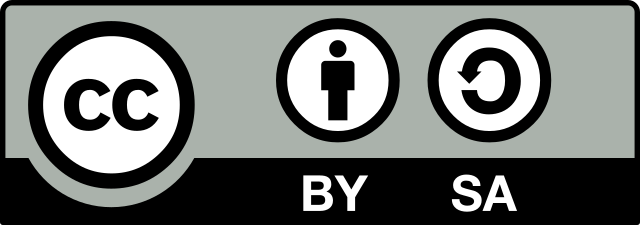
\includegraphics[height = 4ex]{CC.png} 2017 JJ. Merelo, F. Tricas. Este artículo es de acceso libre distribuido bajo los términos
de la Licencia Creative Commons de Atribución, que permite copiar,
distribuir y comunicar públicamente la obra en cualquier medio, sólido
o electrónico, siempre que se acrediten a los autores y fuentes
originales}

\end{multicols}
\end{document}
